\subsection{Ensayos}

\subsubsection{Sin Carga}

Como primer ensayo, se realizaron mediciones de la tensión en el bobinado primario $V_p$, junto con las tensiones del punto medio de cada pata del puente de transistores, $V_p^+$ y $V_p^-$. Todas estas pruebas se realizaron con distintos niveles de desfase entre las señales de las patas del puente, variando ente 0° y 180°, o lo que es lo mismo, variando el ciclo de trabajo del secundario $D_{sec}$ entre 0\% y 100\%.\\

Como esta fue la primer prueba realizada sobre el convertidor CC-CC puente completo, se llevó a cabo sin ningún tipo de carga, dejando los terminales correspondientes a ambos bobinados del transformador a circuito abierto. De esta manera, al no existir circulación de corriente, no se corre el riesgo de destruir algún componente en caso de una falla inesperada del circuito, como podría ser un cortocircuito.\\

El objetivo de este ensayo es relevar el correcto funcionamiento de los circuitos de excitación del puente, compuestos por los dos drivers 2ED21834-S06J. Se debe verificar que sean capaces de disparar los IRFP150, y que funcionen correctamente los circuitos de bootstrap necesarios para activar los transistores del lado alto.\\

\paragraph{Resultados}

\lipsum[1]\\

\begin{figure}[h]
    \centering
    \includegraphics[scale=1.1]{Imagenes/Grafico 90DEG.pdf}
    \caption{Tensión del bobinado primario $V_p$, y tensiones del punto medio de cada pata del puente, $V_p^+$ (azul) y $V_p^-$ (naranja), para una fase de 90°.}
    \label{90DEG}
\end{figure}

\lipsum[4]\\

\subsubsection{Con Carga}

Una vez realizado el ensayo sin carga, y verificado el funcionamiento sin fallas del puente de transistores, se puede proceder a la siguiente prueba. A diferencia del caso anterior, se va a ensayar el convertidor CC-CC completo, conectando el transformador y el inductor de salida $L_f$ a sus terminales correspondientes (ver figura \ref{test_setup}).\\

Como se mencionó en la sección previa, la fuente de laboratorio HP 6010A está encargada de proveer la corriente y tensión necesaria en el primario, mientras que la carga electrónica variable ITECH IT8514B+ se conecta en el terminal de salida del secundario y absorbe la corriente continua de la salida. La fuente se configuró en modo de tensión constante con limitador de corriente variable, y la carga electrónica en modo de resistencia constante.\\

En esta serie de ensayos se miden distintas variables representativas del sistema: tensión de salida $V_{out}$, tensión rectificada $V_{rect}$, corriente de salida $I_{out}$, corriente en el inductor $I_{Lf}$ y tensión del secundario $V_s$. Como en este caso va a existir circulación de corriente, incluso llegando a cargas cercanas a los \SI[]{100}{\watt}, se va a poder observar la respuesta del sistema a grandes circulaciones de corriente, incluido el funcionamiento del rectificador que no se relevó en las pruebas sin carga.\\

\paragraph{Resultados}

\lipsum[2]\\

\begin{figure}[h]
    \centering
    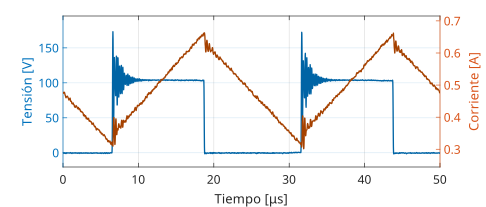
\includegraphics[scale=1]{Imagenes/Grafico DC50 RL100 VIN30.pdf}
    \caption{Tensión rectificada $V_{rect}$ y corriente de inductor $I_{Lf}$ para una carga de \SI[]{100}{\ohm}, ciclo de trabajo de 50\% y tensión de entrada de \SI[]{30}{\volt}.}
    \label{dc50_rL100_vin30}
\end{figure}

\lipsum[3]\\